[Here the theory community will present a discussion of how particles obtain LHC-detector-visible (and beyond) lifetimes in BSM models and describe curated classes of models (including exhaustive citations) that highlight the ways in which the lifetime frontier is an ideal place where new physics could be hiding.

Then each of the experiments will contribute a discussion of why LLP searches are challenging and require non-standard methods.]

Figure~\ref{fig:ATLASCalRatio1} comes from an ATLAS search~\cite{ATLAS-CONF-2016-103}.

\begin{figure}
\centering
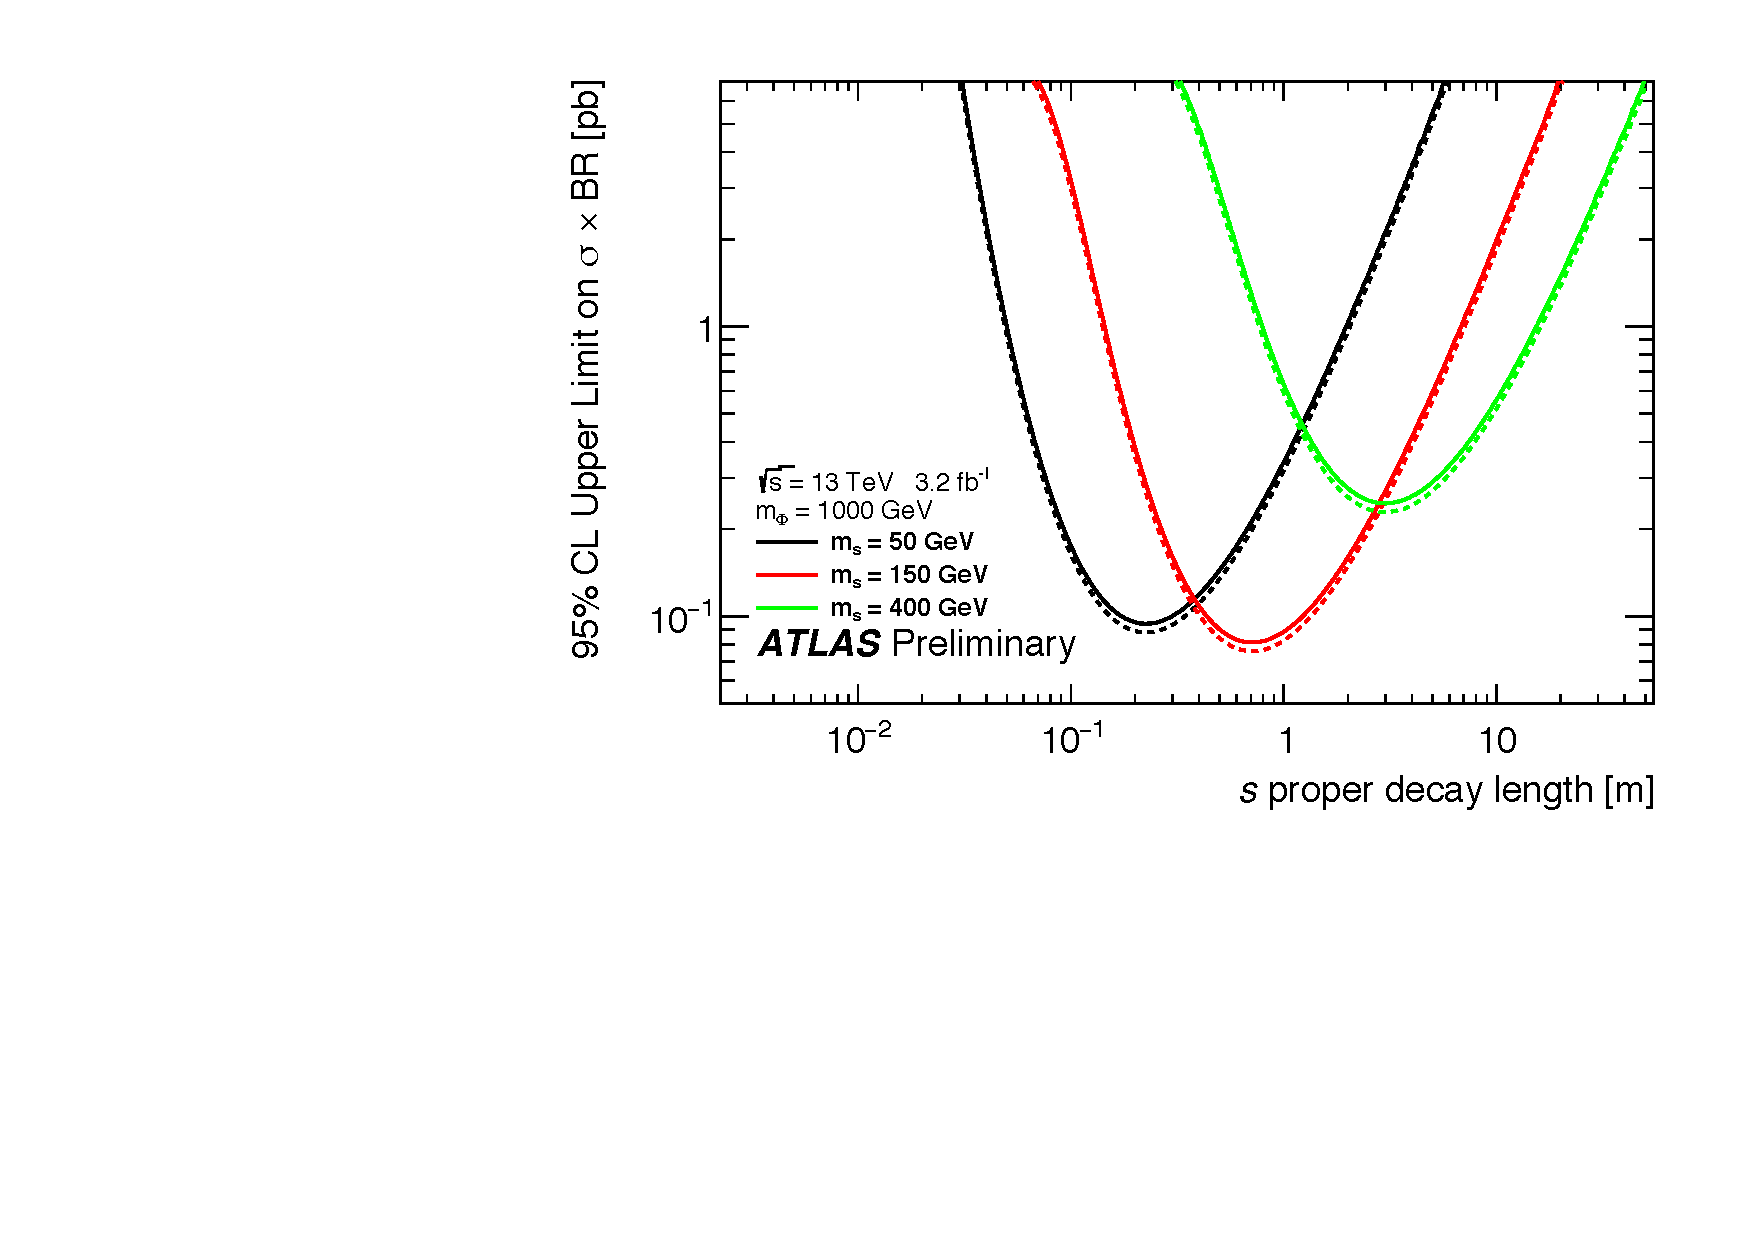
\includegraphics[width=0.95\textwidth]{figures/ATLAS_CalRatio_2016_m1TeV_fig_11c}
%\includegraphics[width=0.95\textwidth]{figures/monojet/width_A}
\caption{ATLAS search for a high-mass scalar $\Phi$ decaying to long-lived scalars, $s$, at $\sqrt{s} = 13$ TeV. From Ref. ~\cite{ATLAS-CONF-2016-103}.}
\label{fig:ATLASCalRatio1}
\end{figure}